\chapter{A Gentle Introduction to Quantum Mechanics}

\graphicspath{{./Figures/Introduction/}}

\section{Introduction}
\begin{quote}
I think I can safely say that nobody understands quantum
mechanics. 
\emph{Richard P. Feynman}

The fundamental laws necessary for the mathematical
treatment of large parts of physics and the whole of chemistry are
thus fully known, and the difficulty lies only in the fact that
application of these laws leads to equations that are too complex to
be solved.
\emph{Paul A. M. Dirac}

In mathematics you don't understand things. You just get used to them.
\emph{Johann von Neumann}
\end{quote}

\noindent The quantum mechanical world can be disorientingly different
from the classical world we are familiar with. Feynman and Dirac's
quotations are strong words from two men who won Nobel prizes for
unraveling the mysteries of quantum mechanics. How are we to rush in
where Feynman and Dirac feared to tread? 

In my opinion, von Neumann summarizes the experience of
learning quantum mechanics very well. Quantum mechanics is only
strange when we try to put it in terms of our classical mechanics
intuition; if we can treat it on its own terms it can be simple and
even beautiful. And to Dirac we might suggest that the availability of
inexpensive computers and 40 years' experience in quantum chemistry
has gone a long way toward, if not \emph{solving} the equations of
quantum mechanics, at least intelligently approximating them.

Quantum chemistry seeks to understand the structure of the world
around us. The world that we see and smell and taste, we do so because
of the quantum chemistry of molecules. Grass is green and blood is
red because of the absorption of light by metalloporphyrin
molecules. The semiconductors that power the microchips that power our
computers switch on and off because of quantum chemical
interactions. Learn a little bit about quantum chemistry and you can
say a lot about the world. This is because electrons are the
\emph{glue} that hold the material world together, and the science
that understands how electrons act as this glue is quantum chemistry.

Moreover, quantum chemistry is a logical stopping point as we cascade
down to smaller and smaller scales. Those areas of physics that
describe scales smaller than the quantum chemistry world (with lengths
on the order of 1 \AA $ = 1\times 10^{-10}$ meter) might be beautiful,
and might offer a deeper appreciation of the symmetry of the laws of
physics, but say nothing more about the nature of the material world
we interact with than does quantum chemistry.

The topic of quantum chemistry is often treated almost as if one needs
the dark secrets of the Rosicrurians to understand the field. Although
I suspect that this misconception does a great deal to satisfy the
egos of quantum chemists, it means that many students who could become
seduced by the intellectual beauty of the field are afraid to take
courses in it. Which is a terrible shame, because never has quantum
chemistry been more important to the technical world.

And so this book seeks to present the material that a student needs to
begin on the path of quantum chemistry. Whenever possible, I seek to
\emph{demystify} the process, to make things as simple as possible. I
have focused on the areas and principles of quantum chemistry that all
students of the field must know, and, as such, I have neglected some
topics, and presented others too briefly. Throughout the book I have
provided extensive citations to other material that will help the
student pursue the topic further.

Although I try to make the material in the book as simple as possible,
students who have not been exposed to college-level General
Chemistry and Calculus courses will probably find the material 
difficult. Also, it will probably be beneficial for students to have
had some exposure to Quantum Mechanics (for example, as it is
typically presented in a sophomore-level Physics Course). For students
who have not had such an introduction, the rest of this chapter
presents the major features of the field as simply as possible.

\section{How the Quantum World Differs from the Classical World}
One of the first indications that something was wrong with the world
of classical physics came in attempts to model \emph{black body
radiation}. Black body radiation refers to the light emitted by a hot
object; it is why a poker left in the fireplace glows red. Indeed, the
color of flames, including the sun, is largely due to black body
radiation. The problem with black body radiation came when physicists
in the late 19th century tried to predict what wave lengths of light
would arise from such a hot object. The equations that Raleigh and
Jeans derived predicted an enormous release of energy that was clearly
wrong. This erroneous prediction was known as the \emph{ultraviolet
catastrophe} (a good name for a glam-rock band if there ever was
one). A crisis arose in physics, because although everyone knew that
Raleigh and Jeans' prediction was wrong, no one knew how to fix it. 

Max Planck and Albert Einstein came to the rescue, fortunately. Planck
found a functional form
\begin{equation}
	\rho(\nu) = \alpha\nu^3\left(\frac{\exp(-h\nu/kT)}
					{1-\exp(-h\nu/kT)}\right)
\label{planck-eq}
\end{equation}
that approximated the energy density $\rho$ of the light
released at a given frequency $\nu$. Einstein provided the physical
interpretation. He reasoned that energy could only be absorbed or
radiated in discrete packets or \emph{quanta} of size $h\nu$. Here $h$
is called \emph{Planck's constant} and has the value $6.6\times10^{-34}
Js$.

Einstein's prediction was a shocking departure. It was as if,
according to Einstein, you could drive your car 55 miles per hour or
57 miles per hour, but there was no way possible that you could drive
your car 56, or 56.2, or 56.3234513, miles per hour, and that you had
to make a discrete jump from 55 to 57 miles per hour. Now, in reality,
the size of the jump is much, much smaller than 2 miles per hour. But
the fact that such a jump, no matter how small, was required ran
contrary to everything the 19th century physicist knew about the
world.

Another mystery at the time was the spectrum of hydrogen. When one
shined light on atomic hydrogen, it would absorb only a few of the
wave lengths. The other wave lengths would pass through the hydrogen
untouched. Neils Bohr took Einstein's idea of energy only being
absorbed or emitted in quanta and proposed a planetary model for the
hydrogen atom. The electrons, he supposed, were negatively charged
particles orbiting the positively charged nucleus like the planets
orbit the sun. The orbits further from the nucleus represent higher
energy states. When an atom absorbs light the electron makes a
\emph{quantum leap} from one of the low orbits to a higher orbit. Only
certain wave lengths of light correspond to the energy difference
between the two states, and only these wave lengths can be absorbed by
the atom. Conversely, when an atom emits light an electron makes
another quantum leap from a state of higher energy to a state of lower
energy. Figure \ref{bohr-atom} sketches the Bohr planetary model for
the hydrogen atom.

\begin{figure}
\begin{center}
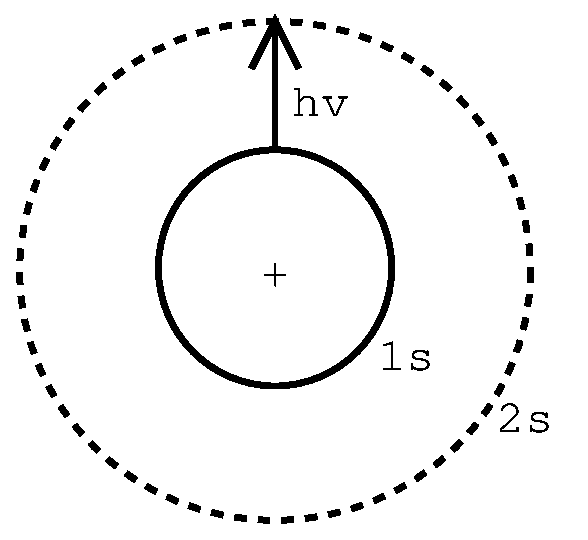
\includegraphics[scale=0.5]{bohr_atom2.eps}
\caption{Bohr's planetary model of the hydrogen atom. The atom can
absorb a photon of frequency $\nu=\frac{E_{2s}-E_{1s}}{h}$ and make a
quantum leap from the $\phi_{1s}$ to the $\phi_{2s}$ orbital.} 
\end{center}
\label{bohr-atom}
\end{figure}

Elegant as Bohr's model of the atom was, it unfortunately failed to
describe more complex properties of atoms such as why they bond
together to form molecules, which is what we are mainly concerned with
in this book. In 1925 Ernest Schrodinger proposed what he called
\emph{wave mechanics}, and Werner Heisenberg proposed he called 
\emph{matrix mechanics}. Both of these theories were later shown to be
equivalent, and are now both subsumed in what is now known as
\emph{quantum mechanics}.

Quantum mechanics solves the \emph{Schrodinger equation}
\begin{equation}
	\hat{H}\psi=E\psi,
\label{simple-schrod-eq}
\end{equation}
which determines everything that can be known about the
atom or molecule we are considering. The Schrodinger equation is an
example of an \emph{eigenvalue equation} (\emph{eigen} is the German
word for \emph{even}). The Schrodinger equation says that there is a
function $\psi$ when acted on by some \emph{operator} $\hat{H}$ yields
the original function $\psi$ times some constant $E$. $\hat{H}$ is
known as the \emph{Hamiltonian operator}, named after
W. R. Hamiltonian, the Astronomer Royal of Ireland, who came very
close to discovering quantum mechanics early in the 19th century. The
Hamiltonian contains all of the sources of energy in our system. We
normally write this as
\begin{equation}
	\hat{H} = \hat{T} + \hat{V}
\end{equation}
where $\hat{T}$ represents the \emph{kinetic energy}---the
energy coming from the momentum of the particles in the system---and
the $\hat{V}$ represents the \emph{potential energy}---the energy (in
molecules) coming from the electrostatic interactions between the
particles in the system. The little hats over the letters indicate
that these terms are \emph{operators} rather than constants. Constants
are just numbers that multiply functions, whereas operators tell us to
do something: take a derivative, multiply it by another number, add
something else to it.

The wave function $\psi$ that is the solution to the Schrodinger
equation provides everything we can know about the system we are
studying. The probability of finding with its particles at 
the coordinates $\{x_1, x_2,  \dots x_N\}$ is given by 
\begin{equation}
	P(x_1,x2,\dots x_N) = |\psi(x_1,x_2,\dots x_N)|^2,
\end{equation}
the square of the wave function. The momentum of the
particles is given by 
\begin{equation}
	\hat{p}\psi = \left(\frac{\hbar}{i}\right)\nabla\psi
\label{momentum}
\end{equation}
where 
\begin{equation}
	\nabla = \frac{\partial}{\partial x},
		\frac{\partial}{\partial y},
		\frac{\partial}{\partial z}
\end{equation}
is the gradient operator---the operator that says to take
the slope in all directions. $\hbar=h/2\pi$ is another form of
Planck's constant.

We've just gone through a lot of mathematics. Hopefully, much of this
rigor will be more understandable after we investigate a real quantum
mechanical system in the next section. But before we do so, let us
comment on the most revolutionary aspects of quantum mechanics. In
classical mechanics, a particle's momentum was computed completely
separately from its position. A car could be driving 30 miles per hour
at the corner of State and Main Streets, or it could be driving 40
miles per hour at the corner of State and Main Streets. Quantum
mechanics tells us that the position and the momentum of a system are
linked, because they both come from the wave function $\psi$. 

The fact that the position and momentum of a particle are linked
together means that if we know the position very exactly, we are
forced to know the momentum a little less exactly, because both of
these quantities come from the same wave function $\psi$, and a wave
function that has a very well defined position has a less well defined
momentum. This trade-off is the \emph{Heisenberg uncertainty
principle}
\begin{equation}
	\delta p\delta x \geq \hbar/2,
\end{equation}
which says that the uncertainty in the measurement of the
momentum $p$ multiplied by the uncertainty in the measurement of the
position $x$ must be greater than one-half Planck's constant. Recall
that Planck's constant is very small, so that the Heisenberg
uncertainty principle does not impose a very large restriction. What
is surprising is not the size of the restriction, but the fact that
there is a restriction at all. Again, like the concepts of quantum
leaps, nothing that the early 20th century physicists had ever seen
before could prepare them for such a development.

Equally strange was the wave nature of matter that the solutions to
the Schrodinger equation implies. In classical mechanics particles are
particles. In quantum mechanics particles often act like waves. Louis
de Broglie distilled this relationship down to the mathematical
expression
\begin{equation}
	\lambda = h/p.
\end{equation}
That is, the wave length associated with a particle is
inversely proportional to its momentum. This relationship explains why
we didn't notice the connection until the late 19th century: for real
world objects like cars and baseballs, the momentum is so large as
compared to Planck's constant $h$ that the wave length is immeasurably
short, and the objects behave as if they had no wave nature at
all. But when objects become small enough, roughly the size of protons
or electrons, we can start to observe their wave nature. Electrons can
interfere with themselves, just as water waves form interference
patterns when they overlap. When electrons pass through small enough
openings, luckily the scale of the spacings in crystals, they can
\emph{diffract}, and we can understand a great deal about the crystal
structure by interpreting the diffraction pattern. Electrons can also
\emph{tunnel}, seep through walls that they shouldn't be able to. The
wave nature of matter tells us that there is a very small probability
that your car will tunnel from your garage to your bedroom while you
sleep. Because cars are large, and thus their wave lengths are very
small, this probability is incredibly small. You could wait many times
the age of the universe without observing it happen. However, there is
some small finite probability that it could occur. Because electrons
are so much smaller than cars, and their wave properties are much more
substantial, we must account for tunneling when we try and predict how
they behave.

One of the real advantages that we as chemists have is that we are
really only concerned with the electrons and nuclei that form
molecules. We will find that molecules are a wonderful arena for the
wierd dance of quantum mechanics to play itself out. As soon as we can
get used to the fact that electrons delocalize over large parts of the
molecule, it becomes very easy to develop a new intuition regarding
the behavior of electrons in molecules.

\section{The Particle in a Box: Analytical Solution}
We will begin our investigation of the behavior of electrons by
looking at what happens when we confine electrons in a small space.
We're really interested in putting an electron in a box. But, since
the math is easier, we will first look at a one-dimensional version of
a box. Of course, electrons aren't one-dimensional, but in the current
exercise we will pretend that they are. 

\begin{figure}
\begin{center}
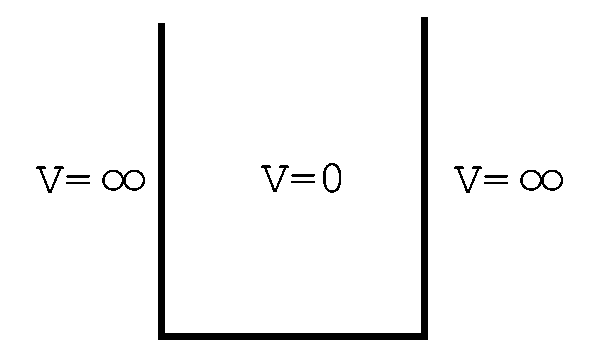
\includegraphics[scale=0.5]{pbox2.eps}
\caption{One dimensional box for an electron. The potential energy is
0 between $x=0$ and $x=L$, and is infinite elsewhere.}
\label{fig-1d-box}
\end{center}
\end{figure}

Figure \ref{fig-1d-box} shows the configuration we are going to
consider. The box is $L$ in length, and since the potential is
infinite at the walls, the electron can never be there. 

To describe this system we must solve the Schrodinger equation, and to
do this we must first determine the Hamiltonian. Classically, the
kinetic energy is given by
\begin{equation}
	T=\frac{p^2}{2m},
\end{equation}
and we can use the same formula in quantum mechanics, by
inserting the expression for $p$ from equation (\ref{momentum}). The 
kinetic energy is then given by
\begin{equation}
	\hat{T}\psi=-\frac{\hbar^2}{2m_e}\nabla^2\psi
\end{equation}
($m_e$ is the mass of the electron). Since we're only doing a one
dimensional problem, we have
\begin{equation}
	\hat{T}\psi=-\frac{\hbar^2}{2m_e}\frac{\partial^2\psi}
		{\partial x^2}.
\end{equation}
As it turns out, we do not have any other sources of energy,
and this expression is the entire Hamiltonian: 
\begin{equation}
	\hat{H}\psi=-\frac{\hbar^2}{2m_e}\frac{\partial^2\psi}
		{\partial x^2}.
\label{pbox_ham}
\end{equation}

Now that we know the form of the Hamiltonian, we begin trying
to solve it. We are looking for a function that has a second
derivative that is a constant times the original function itself. We
note that both $\psi(x) = \sin(x)$ and $\psi(x) = \cos(x)$ meet this
requirement. 

We next look at the boundary condition. Since the potential is
infinite at the walls of the box, the electron can never be there,
which means that the wave function must be zero there. We note that
$\sin(0)=0$, whereas $\cos(0)=1$, which means that $\psi(x)=\sin(x)$
meets the boundary condition at $x=0$. We next write the function is a
slightly more general form, as the function
\begin{equation}
	\psi(x) = A\sin(ax)
\end{equation}
meets all of the requirements that have already been met by
$\psi(x)=\sin(x)$. We will now determine values for $A$ and $a$.

First, we have only used one of the boundary conditions. Recall that
the wave function must be zero at both walls. We have used the wall at
$x=0$ to select the $\sin(x)$ function over the $\cos(x)$
function. We must now chose a value of $a$ such that the function goes
to zero at the $x=L$ wall as well. When $x=L$,
\begin{equation}
	\psi(L) = A\sin(al) = 0.
\end{equation}
Now, the function $\sin(x)$ is zero when
$x=\pi,2\pi,3\pi,\dots$, or generally, $x=n\pi$, where
$n=0,1,2,\dots$. Thus, $al = n\pi$ and $a = \frac{n\pi}{L}$, so that
our wave function is now
\begin{equation}
	\psi(x) = A\sin\left(\frac{n\pi}{L}x\right).
\end{equation}

Recall that the probability of finding an electron at $x$ is given by
$|\psi(x)|^2$. If we integrate the wave function everywhere, we know
we have to find one and only one electron. This requirement is called
\emph{normalization} and leads to
\begin{equation}
	1 = \int_{-\infty}^\infty\left|\psi(x)\right|^2dx
	  = A^2\int_0^L\sin^2\left(\frac{n\pi}{L}x\right)dx.
\label{pbox_norm}
\end{equation}
From a table of integrals we can look up the identify
\begin{equation}
	\int_0^\pi\sin^2(mx)dx = \frac{\pi}{2}.
\end{equation}
Substituting this into equation (\ref{pbox_norm}) yields
\begin{equation}
	1 = A^2 \frac{L}{2}
\end{equation}
and thus,
\begin{equation}
	A = \sqrt{\frac{2}{L}}.
\end{equation}

Our wave function is now
\begin{equation}
	\psi(x) = \sqrt{\frac{2}{L}}\sin\left(\frac{n\pi}{L}x\right).
\label{pbox_psi}
\end{equation}
Recalling that our Hamiltonian is given by equation
(\ref{pbox_ham}), we must solve the equation
\begin{equation}
	E\psi = -\frac{\hbar^2}{2m_e}
		\frac{\partial^2\psi}{\partial x^2}
\end{equation}
Inserting equation (\ref{pbox_psi}) and working through the
derivatives gives
\begin{equation}
	E = \frac{n^2\pi^2\hbar^2}{2m_eL^2}.
\end{equation}
Since we worked so hard for this result, let us take some
time to reflect on some interesting results from this solution. First,
note that the solutions are a function of $n$: we didn't find merely
one solution, we found an entire family of solutions. Secondly, note
that the energy depends upon the square of $n$, which means that as
$n$ increases, the energy levels get further apart. Finally, note that
the energy depends inverseley upon the square of the box length $L$,
which means that as the box gets bigger, the energy becomes more
stable, and subsequent energy levels get closer together.

\begin{figure}
\begin{center}
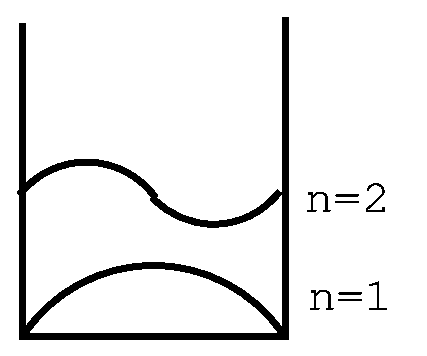
\includegraphics[scale=0.5]{pbox_wfn2.eps}
\caption{Lowest wave functions for an electron in a one-dimensional
box.}
\label{pbox_fig}
\end{center}
\end{figure}

Figure \ref{pbox_fig} shows the lowest wave functions for the electron
in a one-dimensional box.

\section{Solving the Particle in a Box with Grid Points}
In general the problems we will encounter in quantum chemistry do not
have analytical solutions. (When we say a solution is
\emph{analytical} we mean that it has a nice, simple one-line wave
function such as $\psi(x) = A\sin(ax)$.) In fact, the electron in a
box is one of only a very few Hamiltonians that we can solve
analytically. This section will explore the \emph{numerical}
techniques that will let us find approximate solutions using linear
algebra.

Suppose the electron in a one-dimensional box were not solvable
analytically, or suppose it didn't occur to us to try $\sin(x)$ as a
possible solution. We could \emph{numerically approximate} the
solution, by representing it as its value at a finite number of grid
points (the approach we will pursue in this section), or expand in a
finite set of \emph{basis functions} (the approach we will use in much
of the remainder of the book). As we use more points, or more basis
functions, our numerical approximation becomes more and more accurate.

We will employ a principle in quantum chemistry
called the \emph{variational principle} that says that if we do such
an expansion, any solution we find will be higher than the true
energy, and thus the best combination is the one with the lowest
energy. 

We will approximate our wave function as its value at a set of points
$\{x_i\}$. 
\begin{equation}
	\psi(x) \approx c_i x_i
\end{equation}
where $c_i$ are the coefficients that we are going to
adjust to find the lowest energy. Figure \ref{pbox_points}
shows roughly what our approximate wave function might look like.

\begin{figure}
\begin{center}
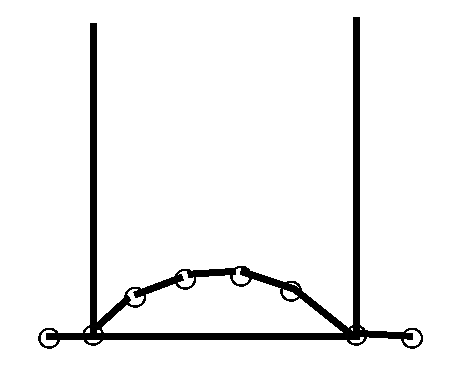
\includegraphics[scale=0.5]{pbox_points.eps}
\caption{Approximation of the wave function by its value at a fixed
number of points. Note that the points continue into
the ``forbidden region'' at either side, but the wave function is zero
in that region.}
\label{pbox_points}
\end{center}
\end{figure}

In order to use such an approximation in the Schrodinger equation, we
must be able to compute the second derivative that is required by the
kinetic energy operator. We will use the \emph{finite difference
approximation}, whereby the first derivative is given by
\begin{equation}
	\frac{df(x_i)}{dx} = \frac{f(x_{i+1})-f(x_{i-1})}{\Delta x}
\end{equation}
and the second derivative is given by
\begin{equation}
	\frac{d^2f(x_i)}{dx^2} = \frac{f(x_{i+1})-2f(x_i)+f(x_{i-1})}
					{\Delta x^2}
\end{equation}	
and $\Delta x=x_i-x_{i-1}=x_{i+1}-x_i$.

To solve the Schrodinger equation, we want to insure that at every
point
\begin{equation}
  -\frac{\hbar^2}{2m_e}\frac{d^2\psi(x_i)}{dx^2} + V(x_i) =
   E\psi(x_i).
\label{finite-schrod}
\end{equation}	
We can solve these equations by setting them up in a matrix
equation. If we wish to find the eigenfunctions of the second
derivative operator alone, we could solve a set of equations that look
like: 
\begin{equation}
  \left[\begin{array}{ccccc}
    -\frac{2}{\delta^2}&\frac{1}{\delta^2}&&&\\
    \frac{1}{\delta^2}&-\frac{2}{\delta^2}&\frac{1}{\delta^2}&&\\
     &\frac{1}{\delta^2}&-\frac{2}{\delta^2}&\frac{1}{\delta^2}&\\
     &&&\ddots&\\
     &&&\frac{1}{\delta^2}&-\frac{2}{\delta^2}\\   
  \end{array}\right]
  \left[\begin{array}{c}
  c_1\\c_2\\c_3\\\vdots\\c_n
  \end{array}\right]
  = E
  \left[\begin{array}{c}
  c_1\\c_2\\c_3\\\vdots\\c_n
  \end{array}\right]
\label{lapl-mat}
\end{equation}
These matrix equations are known as eigenvalue equations. The
correspondence between the differential equations known as eigenvalue
equations (for example, equation (\ref{simple-schrod-eq})) and their
finite matrix representation is a difficult one to get an intuitive
feeling for. The next section gives a brief introduction to matrix
equations. 

\section{Matrix Equations}
Vectors and matrices are one- and two-dimension arrays of
variables; they are useful because by manipulating matrices and
vectors we can often obtain an entire family of solutions. The field
of \emph{linear algebra} deals with solving matrix and vector
equations. One particularly useful result of rewriting equations in
matrix/vector form is that we can then use standard linear algebra
packages such as the LAPACK program library \cite{laug} to obtain
solutions to the equations on a computer.

A matrix is a two-dimensional array of numbers:
\begin{equation}
	\matvec{A} = 
		\left[\begin{array}{cccc}
			A_{11} & A_{12} & A_{13} & A_{14} \\
			A_{21} & A_{22} & A_{23} & A_{24} \\
			A_{31} & A_{32} & A_{33} & A_{34} \\
			A_{41} & A_{42} & A_{43} & A_{44} \\
			A_{51} & A_{52} & A_{53} & A_{54} \\
		\end{array}\right]
\end{equation}
where here the matrix \matvec{A} is said to have 4
\emph{columns} and 5 \emph{rows}. 

A vector is a matrix with only one column:
\begin{equation}
	\matvec{b} = \left[\begin{array}{c}
			b_1 \\ b_2 \\ b_3 \\ b_4
			\end{array}\right].
\end{equation}
Here the vector \matvec{b} has 4 \emph{rows}.

We can define addition and subtraction on matrices as well:
\begin{equation}
	\matvec{A} + \matvec{B} = 
		\left[\begin{array}{cccc}
	A_{11}+B_{11}  & A_{12}+B_{12}  & A_{13}+B_{13}  & A_{14}+B_{14}  \\
	A_{21}+B_{21}  & A_{22}+B_{22}  & A_{23}+B_{23}  & A_{24}+B_{24}  \\
	A_{31}+B_{31}  & A_{32}+B_{32}  & A_{33}+B_{33}  & A_{34}+B_{34}  \\
	A_{41}+B_{41}  & A_{42}+B_{42}  & A_{43}+B_{43}  & A_{44}+B_{44}  \\
	A_{51}+B_{51}  & A_{52}+B_{52}  & A_{53}+B_{53}  & A_{54}+B_{54}  \\
		\end{array}\right]
\end{equation}
which of course only works if \matvec{A} and \matvec{B} have the same
number of rows and columns. Similarly, vector sums are given by
\begin{equation}
	\matvec{a}+\matvec{b} = \left[\begin{array}{c}
			a_1+b_1 \\ a_2+b_2 \\ a_3+b_3 \\ a_4+b_4
			\end{array}\right]
\end{equation}
and the vectors must have the same number of rows.

We define the product of a scalar $\alpha$ and a matrix \matvec{B} as
\begin{equation}
	\alpha\matvec{B} = 
		\left[\begin{array}{cccc}
	\alpha B_{11}  & \alpha B_{12}  & \alpha B_{13}  & \alpha B_{14}  \\
	\alpha B_{21}  & \alpha B_{22}  & \alpha B_{23}  & \alpha B_{24}  \\
	\alpha B_{31}  & \alpha B_{32}  & \alpha B_{33}  & \alpha B_{34}  \\
	\alpha B_{41}  & \alpha B_{42}  & \alpha B_{43}  & \alpha B_{44}  \\
	\alpha B_{51}  & \alpha B_{52}  & \alpha B_{53}  & \alpha B_{54}  \\
		\end{array}\right].
\end{equation}
We define the product of two matrices
$\matvec{C}=\matvec{A}\times\matvec{B}$ as
\begin{equation}
	C_{ij} = \sum_k^N A_{ik}B_{kj}.
\end{equation}
Here $N$ is equal to the number of columns of \matvec{A} and the
number of rows of \matvec{B}; if the number of columns of the first
matrix is equal to the number of rows of the second matrix we can
multiply them. When we multiply a $M\times N$ matrix by a $N\times P$
matrix we obtain a $M\times P$ matrix. Since vectors are just matrices
with one column, we can multiply a matrix by a vector $\matvec{c} =
\matvec{A}\times\matvec{b}$ if the number of columns of \matvec{A} is
equal to the number of rows of \matvec{b}. When we multiply a $M\times
N$ matrix by a $N$-vector, we obtain an $M$ vector. 

Note that in general matrix multiplication does not
\emph{commute}. That is, 
\begin{equation}
	\matvec{A}\times\matvec{B} \neq \matvec{B}\times\matvec{A}.
\end{equation}

In this book, we will write matrices with an uppercase emboldened
letter, e.g. \matvec{A}, and vectors with a lowercase emboldened
letter, e.g. \matvec{b}.

We define the \emph{transpose} of a matrix with the superscript
$^\dag$. The transpose of a matrix is obtained by switching the rows
and columns. That is, 
\begin{equation}
	\matvec{A}^\dag = 
		\left[\begin{array}{ccccc}
			A_{11} & A_{21} & A_{31} & A_{41} & A_{51}\\
			A_{12} & A_{22} & A_{32} & A_{42} & A_{52}\\
			A_{13} & A_{23} & A_{33} & A_{43} & A_{53}\\
			A_{14} & A_{24} & A_{34} & A_{44} & A_{54}\\
		\end{array}\right];
\end{equation}
when we take the transpose of a $5\times 4$ matrix we obtain a
$4\times 5$ matrix. The transpose of a (column) vector is a \emph{row
vector}, and corresponds to a matrix with only one row.

Closely related to the transpose of a matrix is the
\emph{adjoint}. The adjoint of the matrix \matvec{A} is written
$\matvec{A}^*$, and the values are given by
\begin{equation}
	\matvec{A}^* = 
	\left[\begin{array}{ccccc}
		A_{11}^* & A_{21}^* & A_{31}^* & A_{41}^* & A_{51}^*\\
		A_{12}^* & A_{22}^* & A_{32}^* & A_{42}^* & A_{52}^*\\
		A_{13}^* & A_{23}^* & A_{33}^* & A_{43}^* & A_{53}^*\\
		A_{14}^* & A_{24}^* & A_{34}^* & A_{44}^* & A_{54}^*\\
	\end{array}\right];
\end{equation}
where $A_{ij}^*$ represents the \emph{complex conjugate} of
$A_{ij}$. If $A_{ij}$ is complex, that is, if it has both a real and
imaginary part given by $A_{ij} = a+ib$, $A_{ij}^* = a-ib$. Obviously,
if \matvec{A} is real, $\matvec{A}^* = \matvec{A}^\dag$.

A special type of matrix we will encounter in quantum mechanics is
called a \emph{Hermitian matrix}. A Hermitian matrix is
\emph{self-adjoint}, $\matvec{A} = \matvec{A}^*$. If all of the
values of \matvec{A} are real, the matrix is \emph{symmetric},
$\matvec{A} = \matvec{A}^\dag$. 

% determinant
% linear solve

The most common type of matrix problem we will come across in quantum
mechanics is the \emph{eigenvalue equation}, which is the linear algebra
version of equation (\ref{simple-schrod-eq}). In this format, given a
matrix \matvec{A}, we wish to find the family of solution vectors
\matvec{x} and scalars $\lambda$ where
\begin{equation}
	\matvec{A}\matvec{x} = \lambda\matvec{x}.
\end{equation}
Solving an eigenvalue equation like this is often referred to as
\emph{diagonalization} because we find a transformation that will make
\matvec{A} into a diagonal matrix to solve the equations. The scalar
values $\lambda$ are known as the \emph{eigenvalues} of \matvec{A},
and the vectors \matvec{x} are known as the \emph{eigenfunctions} or
\emph{eigenvalues} of \matvec{A}.

One interesting property of Hermitian and symmetric matrices is that
all of their eigenvalues are real. Additionally, for symmetric
matrices the eigenvectors are also real.

We will discuss other problems in linear algebra as we encounter them.

\section{Solving the Matrix Equations for the Particle in a Box}
We now have enough information to begin considering solutions to the
numerical one-dimensional Schrodinger equation give in equation
(\ref{finite-schrod}). First, let's set some parameters for the
problem. We will solve for the energy levels of an electron in a box
of length 1 atomic unit. \emph{Atomic units} are chosen so that the
mass of an electron ($9.1\times10^-31$ kg) is the mass unit, the
electron charge ($4.8\times10^{-10}$ esu) is the charge unit, and the
Bohr radius (0.529 \AA) is the length unit, and the \emph{hartree}
(627.51 kcal/mol) is the energy unit. These units are convenient
because in atomic units $\hbar=1$, and the Schrodinger equation is
greatly simplified.

We will space points at {0, 0.1, 0.2, 0.3, 0.4, 0.5, 0.6, 0.7, 0.8,
0.9, 1.0}. The points at 0.0 and 1.0 will be in the forbidden
region. Technically the potential is infinite in this region. Since
computers can't handle infinite numbers, we will set the potential to
be 100 atomic units of energy (also known as \emph{Hartrees}), an
enormous amount of energy (it takes only $\approx$ 0.1 -- 0.2 Hartrees
to break a typical chemical bond).

Our Hamiltonian now looks like
\begin{equation}
H = \frac{1}{\delta^2}\left[
\begin{array}{ccccccccccc}
100&-\frac{1}{2}&&&&&&&&&\\
-\frac{1}{2}&1&-\frac{1}{2}&&&&&&&&\\
&-\frac{1}{2}&1&-\frac{1}{2}&&&&&&&\\
&&-\frac{1}{2}&1&-\frac{1}{2}&&&&&&\\
&&&-\frac{1}{2}&1&-\frac{1}{2}&&&&&\\
&&&&-\frac{1}{2}&1&-\frac{1}{2}&&&&\\
&&&&&-\frac{1}{2}&1&-\frac{1}{2}&&&\\
&&&&&&-\frac{1}{2}&1&-\frac{1}{2}&&\\
&&&&&&&-\frac{1}{2}&1&-\frac{1}{2}&\\
&&&&&&&&-\frac{1}{2}&1&-\frac{1}{2}\\
&&&&&&&&&-\frac{1}{2}&100\\
\end{array}
\right]
\label{conf-el-ham}
\end{equation}
and the terms not listed are zero.
Here we are neglecting the kinetic energy terms in the forbidden
region, because we assume that the magnitude of this term will be far
less than the potential term.

We solve equation (\ref{conf-el-ham}) by using a computer program to
compute the eigenvalues and eigenvectors of the matrix. Appendix
\ref{conf-el-prog} has some simple programs to compute these values,
but here we show examples of the solutions.

\begin{table}
\caption{Comparison of the numeric and analytical energies (in
Hartrees) of the lowest three states of the particle in a box.}
\label{conf-el-compare}
\begin{center}
\begin{tabular}{cccc}\\ \hline\hline
$n$ & $E_1$ & $E_2$ & $E_3$ \\ \hline
11 & 4.885 & 19.06 & 41.16 \\
21 & 4.920 & 19.56 & 43.56 \\
41 & 4.930 & 19.69 & 44.19 \\
81 & 4.933 & 19.72 & 44.35 \\
161 & 4.934 & 19.73 & 44.39 \\
Analytical & 4.935 & 19.74 & 44.41 \\ \hline\hline
\end{tabular}
\end{center}
\end{table}

Table \ref{conf-el-compare} compares the analytical and numeric
energies of the lowest three eigenstates of the particle in a box
problem. By the time we have use 161 points we are making decent
approximations to the exact results.

\begin{figure}
\begin{center}
\includegraphics[scale=0.4,angle=270]{conf_el.eps}
\end{center}
\caption{Comparison of the numeric (points) and exact (line) solutions
for the most stable wave function for the particle in a box. Even with
only 11 points, the functions are nearly indistinguishable.}
\label{conf-el-fig}
\end{figure}

Figure \ref{conf-el-fig} compares the lowest energy wave functions for
the numeric and analytical techniques.

\section{Solving Other One Dimensional Hamiltonians with Grid Points}
It only took us a page to write down the analytical solution to the
particle in a box, and it took us many times as long to write down the
numerical solution. Why should we bother with numerical solutions?

There are only three quantum mechanical problems that we can solve
analytically---the particle in a box that we already saw, the harmonic
oscillator, and the Hydrogen atom. Whereas we can use the simple code
that we just worked out and solve almost \emph{any} one-dimensional
problem that nature throws at us. This section will explore some of
the systems that are most relevant to Chemistry.

\begin{figure}
\begin{center}
\includegraphics[scale=0.5,angle=270]{harmonic.eps}
\end{center}
\caption{Lowest three eigenvectors of the harmonic oscillator with
potential $V(x)=50x^2$. The same code that computed the particle in a
box problem can be used with a different potential to compute the new
problem.}
\label{harmonic-plot}
\end{figure}

Figure \ref{harmonic-plot} shows the three lowest eigenvectors of the
harmonic oscillator with the potential $V(x)=50x^2$.

%\subsection{Double Well}
% Symmetric and asymmetric

\begin{figure}
\begin{center}
\includegraphics[scale=0.5,angle=270]{coulomb.eps}
\end{center}
\caption{Lowest three eigenvectors of the Coulomb potential
$V(x)=\frac{1}{|x|}$. The potential and the energy of the lowest
eigenvector are not drawn to scale for simplicity.}
\label{coulomb-plot}
\end{figure}

Figure \ref{coulomb-plot} shows the three lowest eigenvectors of the
Coulomb potential $V(x)=\frac{1}{|x|}$. This is a one-dimensional
version of the electron-nuclear potential seen in the hydrogen
atom. Note that, in contrast to the rounded wave functions the
harmonic oscillator had at the origin, the Coulomb wave functions have
cusps, a result of the singularity in the potential at the
origin. Again, the same code is used to solve this potential as was
used in the other one-dimensional problems.

The reader will note that the matrices we have derived for the kinetic
energy, potential energy, and the total Hamiltonian are all symmetric,
$\matvec{A} = \matvec{A}^\dag$.
This relationship isn't accident, we can show that the matrices
derived from all quantum mechanical operators corresponding to
observable properties are Hermitian. 


\section{Basis Set Expansions}
In the previous section we saw the utility of expanding our wave
function in some sort of a numerical approximation. In that section we
approximated the wave function as its values at a number of different
points.  As the we use more and more points this approximation becomes
more exact. This is a useful approximation for one-dimensional
potentials, but becomes less effective in two and higher dimensions.

The Schrodinger equation determines the optimal shape for the wave
function. By expanding the wave function in a finite set of points,
the problem of optimizing the wave function shape is transformed into
a matrix problem, which can be easily solved on a computer.

For molecular systems we will expand in a \emph{basis set}. Basis
functions are primitive three-dimensional shapes; when we expand the
wave function in a set of basis functions we once again obtain a
matrix equation that can be easily solved. Subsequent chapters will
discuss basis functions and the resulting matrix equations in more
detail.

The most common type of basis function used in quantum chemistry is
the \emph{Gaussian basis function}, which has the form
\begin{equation}
 \chi(x;x_0) = N\exp\{-\alpha(x-x_0)^2\}
\end{equation}
in one dimension. Here $N$ is the normalization constant, and $x_0$ is
the center of the function. Gaussian functions have a number of
properties that make them useful for quantum chemistry. The first is
that the product of two Gaussians on different centers is another
Gaussian centered somewhere in between. That is,
\begin{equation}
 \exp\{-\alpha(x-x_a)^2\}\exp\{-\beta(x-x_b)^2\} = 
   \exp\left\{\frac{-\alpha\beta(x_a-x_b)^2}{\gamma}\right\}
   \exp\{-\gamma (x-x_c)^2\},
\end{equation}
where
\begin{equation}
	\gamma = \alpha+\beta,
\end{equation}
\begin{equation}
	x_c = \frac{\alpha x_a+\beta x_b}{\gamma}.
\end{equation}
This property greatly simplifies the matrix elements we need to
calculate.

If we want to use gaussian basis functions to solve the particle in a
box, we need to work out several different types of matrix elements to
go into the matrix form of the Schrodinger equation. The easiest of
these elements is the overlap matrix elements
\begin{eqnarray}
 S_{ij} &=& \int \chi_i(x)\chi_j(x)dx \\
  &=&N^2\int\exp\{-\alpha_i(x-x_i)^2\}\exp\{-\alpha_j(x-x_j)^2\}dx\\
  &=&N^2\exp\left\{\frac{\alpha_i\alpha_j(x_i-x_j)^2}{\gamma}\right\}
        \int\exp\{-\gamma(x-x_c)^2\}dx\\
  &=&\exp\left\{\frac{\alpha_i\alpha_j(x_i-x_j)^2}{\gamma}\right\}
\end{eqnarray}
which, if we stipulate $\alpha_i=\alpha_j=\alpha$, simplifies to
\begin{equation}
 S_{ij} = \exp\{\alpha(x_i-x_j)^2\}.
\end{equation}
The potential energy matrix elements are given by
\begin{eqnarray}
 V_{ij} &=& \int \chi_i(x)V(x)\chi_j(x)dx \\
  &=&N^2\int\exp\{-\alpha_i(x-x_i)^2\}V(x)\exp\{-\alpha_j(x-x_j)^2\}dx\\
  &=&N^2\exp\left\{\frac{\alpha_i\alpha_j(x_i-x_j)^2}{\gamma}\right\}V(x_c)
        \int\exp\{-\gamma(x-x_c)^2\}dx\\
  &=&\exp\left\{\frac{\alpha_i\alpha_j(x_i-x_j)^2}{\gamma}\right\}V(x_c)\\
  &=&\exp\{\alpha(x_i-x_j)^2\}V\left(\frac{x_i+x_j}{2}\right),
\end{eqnarray}
assuming that V(x) is a constant-valued function such as in the
particle in a box, where it is either 0 or $\infty$.

The kinetic energy matrix elements are the most difficult. These are
given by
\begin{eqnarray}
 T_{ij}&=& -\frac{1}{2}\int \chi_i(x)\frac{d^2}{dx^2}\chi_j(x)dx \\
  &=&-\frac{N^2}{2}\int\exp\{-\alpha_i(x-x_i)^2\}\frac{d^2}{dx^2}
         \exp\{-\alpha_j(x-x_j)^2\}dx\\
  &=&N^2\int\exp\{-\alpha(x-x_i)^2\}(\alpha-2\alpha^2(x-x_j)^2)\nonumber\\
     &&   \times\exp\{-\alpha(x-x_j)^2\}dx\\
  &=&N^2\alpha\int\exp\{-\alpha(x-x_i)^2\}\exp\{-\alpha(x-x_j)^2\}\nonumber\\ 
    &&-2N^2\alpha^2\int\exp\{-\alpha(x-x_i)^2\}(x-x_i)^2\nonumber\\
    &&\times\exp\{-\alpha(x-x_j)^2\}dx\\
  &=&\alpha\exp\{\alpha(x_i-x_j)^2\}
    -2N^2\alpha^2\exp\{\alpha(x_i-x_j)^2\}\times\nonumber\\
    &&\int(x-x_i)^2\exp\{-\alpha(x-x_c)^2\}dx.
\end{eqnarray}
The problem with the last equation is that it is the product of
functions centered about two different centers.
We must expand the $(x-x_i)^2$ term in a binomial series about $x_c$
to put the equation in a form we can integrate.

% Correct form of the kinetic energy operator

Now that we have all of the matrix elements we need for the particle 
in a box we can solve the equations. The form of the Schrodinger
equation is
\begin{equation}
 (\matvec{T}+\matvec{V})\matvec{c} = \matvec{S}\matvec{c}E,
\end{equation}
which, because of the presence of the overlap matrix \matvec{S}, is a 
little more complex than the form we solved using the grid point method. 
With grid points we didn't have to worry about overlap, but with Gaussian
functions we do. This transforms the normal matrix eigenvalue equation 
into a generalized eigenvalue problem. This, too, may be solved using 
standard routines from linear algebra packages.

% Plot out solutions of this equation, compare to the others.

\section{Suggestions for Further Reading}
Volume III of Feynman's \emph{The Feynman Lectures on Physics}
\cite{Feynman65} presents a careful and thoughtful introduction to
quantum mechanics. Pauling's \emph{The Nature of the Chemical Bond}
\cite{Pauling60} is a magnificent introduction to quantum mechanics in
chemistry. For more mathematical treatments of the subject, both
Dirac's \emph{The Principles of Quantum Mechanics} \cite{Dirac57} and
von Neumann's \emph{Mathematical Foundations of Quantum Mechanics}
\cite{VonNeumann55} offer detailed discussion of the quantum
mechanical theory that underpins the material in this
section, and are both remarkably easy to read. 
